%%%%%%%%%%%%%%%%%%%%%%%%%%%%%%%%%%%%%%%%%%%%%%%%%%%%%%%%%%%%%%%%%%%%%%%%
% PACKAGES
%%%%%%%%%%%%%%%%%%%%%%%%%%%%%%%%%%%%%%%%%%%%%%%%%%%%%%%%%%%%%%%%%%%%%%%%

\documentclass[11pt,a4paper]{article}
\usepackage[czech]{babel}
\usepackage[utf8]{inputenc}
\usepackage[T1]{fontenc}
\usepackage{lmodern}
\usepackage{textcomp}
\usepackage{geometry}
\usepackage[hidelinks]{hyperref}
\usepackage{bookmark}
\usepackage{enumitem}
\usepackage{parskip}
\usepackage{titlesec}
\usepackage{graphicx}
\usepackage{float}
\usepackage{tabularx,array}
\usepackage{booktabs} 
\usepackage{comment}
\usepackage{siunitx}
\usepackage{threeparttable}
\usepackage[format=hang]{caption}

\geometry{margin=2.2cm}
\setlist{nosep,leftmargin=2em}

%%%%%%%%%%%%%%%%%%%%%%%%%%%%%%%%%%%%%%%%%%%%%%%%%%%%%%%%%%%%%%%%%%%%%%%%
% COMMANDS CONFIG
%%%%%%%%%%%%%%%%%%%%%%%%%%%%%%%%%%%%%%%%%%%%%%%%%%%%%%%%%%%%%%%%%%%%%%%%

% Definice subsubsubsection
\titleclass{\subsubsubsection}{straight}[\subsubsection]
\newcounter{subsubsubsection}[subsubsection]
\renewcommand\thesubsubsubsection{\thesubsubsection.\arabic{subsubsubsection}}
\titleformat{\subsubsubsection}
  {\normalfont\normalsize\bfseries}{\thesubsubsubsection}{1em}{}
\titlespacing*{\subsubsubsection}{0pt}{1.25ex plus 1ex minus .2ex}{0.75ex plus .2ex}

% Definice subsubsubsubsection
\titleclass{\subsubsubsubsection}{straight}[\subsubsubsection]
\titleformat{\subsubsubsubsection}
  {\normalfont\normalsize\bfseries}{}{0pt}{}%
\titlespacing*{\subsubsubsubsection}
  {0pt}{1.25ex plus 1ex minus .2ex}{0pt}

% Nastavení hloubky číslování a obsahu
\setcounter{secnumdepth}{4} % Hloubka číslování
\setcounter{tocdepth}{4}    % Hloubka obsahu

% Přidání subsubsubsection do obsahu
\makeatletter
    \newcommand{\l@subsubsubsection}{\@dottedtocline{4}{7em}{4em}}
    % subsubsubsubsection z obsahu úplně vyhodíme (i kdyby bylo něco v .toc)
    \newcommand*\l@subsubsubsubsection[2]{}
    
    % Mapování úrovní pro správné záložky
    \providecommand*{\toclevel@subsubsubsection}{4}
    \providecommand*{\toclevel@subsubsubsubsection}{5}
\makeatother

% Zalamování v tabulkách
\newcolumntype{L}{>{\raggedright\arraybackslash}X}
\newcolumntype{P}{>{\ttfamily\raggedright\arraybackslash}X} 


%%%%%%%%%%%%%%%%%%%%%%%%%%%%%%%%%%%%%%%%%%%%%%%%%%%%%%%%%%%%%%%%%%%%%%%%
% DOCUMENT START
%%%%%%%%%%%%%%%%%%%%%%%%%%%%%%%%%%%%%%%%%%%%%%%%%%%%%%%%%%%%%%%%%%%%%%%%

\begin{document}

%%%%%%%%%%%%%
% Title page
%%%%%%%%%%%%%

\begin{titlepage}
    \begin{center}
        \Huge{\textsc{Vysoké učení technické v~Brně}\\}
        \vspace{0.5em}
        \huge\textsc{Fakulta informačních technologií}\\
        \vspace{\stretch{0.382}}
        {\huge Mikroprocesorové a vestavěné systémy (IMP)\,--\,Projekt\\
                \vspace{0.6em}
                Hra na displeji\,--\,Bee Pollination\\}
        \vspace{\stretch{0.618}}
    \end{center}
    \Large 2025 \hfill Jan Kalina (xkalinj00)
\end{titlepage}

\newpage


%%%%%%%%%%%%%%%%%%%%
% Table of contents
%%%%%%%%%%%%%%%%%%%%

{
    \hypersetup{linkcolor=black}
    \tableofcontents
}

\newpage


%%%%%%%%%%%%%%%%%%%%%%%%%%%%%%%%%%%%
% Introduction and Conceptual model
%%%%%%%%%%%%%%%%%%%%%%%%%%%%%%%%%%%%

\section{Úvod}

Cílem pro jektu je vytvořit jednoduchou hru na displeji pro mikrokontrolér ESP32\cite{reference} využívající potenciometrických vlastností joysticku. V rámci projektu jsem se rozhodl vytvořit
jednoduchou 2D arkádovou hru s názvem \emph{Bee Pollination} (\uv{Opylování}). Moje realizace demonstruje propojení více periferií\,--\,joysticku, grafického OLED displeje SSD1306 a časovače -- při
tvorbě interaktivní aplikace. Z hlediska hardware je k realizaci projektu využitý \emph{joystick}, \emph{OLED displej SSD1306} a vývojová deska \emph{WeMos D1 R32} založená na čipu \emph{ESP32}. 

Tématem hry je opylování květin. Hráč ovládá malou včelu, která přenáší pyl z jedné květiny na druhou v časovém limitu 60 sekund. Cílem je dosáhnout co nejvyššího skóre úspěšným
opylením co nejvíce květin v daném čase. Hra přitom simuluje různé překážky a vylepšení inspirované reálným světem. Na herní ploše se náhodně objevují predátoři (pavouci), kterým je
třeba se vyhnout, kapky deště zpomalující pohyb včely a také vylepšení (\uv{power-upy}) v podobě štítu (dočasná ochrana před pavouky) a medu (dočasné zrychlení). Projekt tak zábavnou
formou demonstruje práci s mikrokontrolérem a jeho periferiemi -- analogovými vstupy, digitálními vstupy/výstupy, sběrnicí $\text{I}^2\text{C}$ a grafickým OLED displejem.
Hra je implementována jazyce C s využitím vývojového frameworku \texttt{ESP-IDF} od Espressifu, který poskytuje potřebné softwarové knihovny pro práci s hardware (pro ADC, $\text{I}^2\text{C}$ i řízení displeje).

\subsection{Video}

Demonstrační video (FullHD) je dostupné na mém Google Disku v této sdílené složce:\\ \href{https://drive.google.com/drive/folders/1icxXEqtqzk53VCFcV1F5xSe-IhUn7lpO?usp=drive_link}{\texttt{https://drive.google.com/drive/folders/1icxXEqtqzk53VCFcV1F5xSe-IhUn7lpO?usp=drive\_link}}

nebo také na platformě YouTube (lepší kvalita i bez stažení) pod tímto odkazem:\\ \href{https://youtu.be/jT92WX7A0JY}{\texttt{https://youtu.be/jT92WX7A0JY}}

\section{Použité prostředky}

\subsection{Vývojová deska WeMos D1 R32}

Vývojová deska \emph{WeMos D1 R32}\cite{wemos} je základem celho projektu. Je to deska s mikrokontrolérem \emph{ESP32} v provedení kompatibilním s platformou Arduino UNO (\emph{Pozn.: Arduino nebylo 
při realizaci projektu využito}). Použitý modul se pyšní dvoujádrovým 32bitovým procesorem a integrovanou podporou Wi-Fi/Bluetooth, napájecí a komunikační rozhraní (Micro USB převodník UART).  Všechny vstupy/výstupy (GPIO) ESP32 pracují na úrovni 3,3\,V\,--\,deska umí poskytnout výstup 5\,V (např. pro 
napájení periferií), avšak jakákoliv logická pinová signalizace nad 3,3\,V by mohla mikrokontrolér nenávratně poškodit. ESP32 nabízí celkem 34 programovatelných GPIO pinů, z
toho 18 lze použít jako analogové vstupy do 12bitového ADC (dvě nezávislé ADC jednotky).\cite{datasheet} Na desce D1 R32 je těchto analogových pinů vyvedeno 6 jako \uv{analog in}. Některé piny 
(\texttt{GPIO34}--\texttt{GPIO39}) jsou pouze vstupní a neobsahují ani interní pull-up/pull-down rezistory, což je důležité zohlednit při jejich použití. Digitální piny naopak mohou 
fungovat jako vstupy i výstupy (\texttt{GPIO0}--\texttt{GPIO33}) a podporují řadu rozhraní (UART, SPI, $\text{I}^2\text{C}$, PWM atd.). Na obrázku níže je znázorněno rozmístění pinů na 
použité desce D1 R32.

\begin{figure}[H]
    \centering
    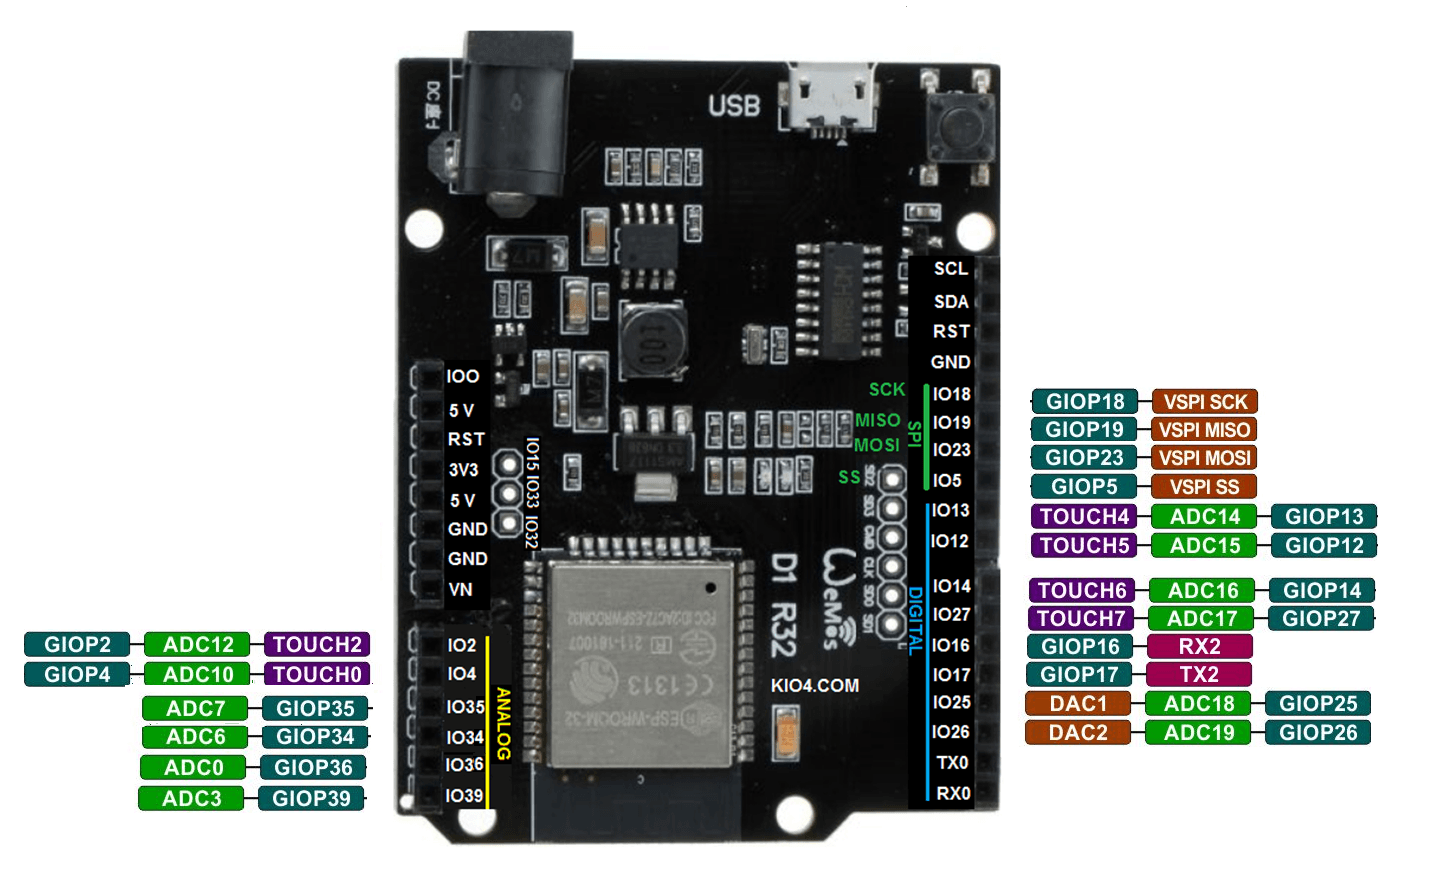
\includegraphics[width=\linewidth]{Obrázky/pinout.png}
    \caption{Pinout diagram\,--\,digitální I/O (modře), analogové vstupy ADC (žlutě), aj.}
    \label{fig:pinout}
\end{figure}

\subsection{Analogový joystick}

K realizaci mi byl přidělen proporcionální dvouosý joystick (typicky používaný v herních ovladačích). Slouží jako hlavní vstup pro ovládání hry. Fyzicky jde o modul se dvěma ortogonálně
umístěnými potenciometry a návratovou pružinou. Vychýlením páčky se mění děliče napětí a poskytují na výstupech dvě analogová napětí úměrná vodorovnému (X) a svislému (Y) posunu páčky. 
Joystick byl napájen 3,3\,V z desky ESP32 a jeho výstupy byly připojeny na dva analogové vstupní piny mikrokontroléru (využity dva kanály \texttt{ADC1} -- kanály 6 a 7). ESP32 převádí vstupní
napětí přes interní 12bitový SAR ADC\,--\,hodnoty potenciometru 0--3,3\,V jsou repzrezentovány jako hodnoty v číselném rozsahu 0--4095. Kromě analogových os má joystick i integrované
tlačítko (sepne při stlačení páčky dolů). Toto tlačítko bylo zapojeno na digitální vstup ESP32 (konkrétně \texttt{GPIO27}) v režimu vstupu s interním pull-up rezistorem, takže v nestlačeném
stavu drží logickou \uv{$1$} a při stisknutí se pin uzemní tím se nastaví logická hodnota \uv{$0$}. Toto tlačítko slouží ve hře k zahájení hry nebo k pozastavení/obnovení nové hry.

Při startu hry probíhá krátká kalibrace středové polohy (zprůměrování několika vzorků), aby bylo možné počítat relativní výchylku v obou směrech. Za běhu hry se analogové hodnoty periodicky čtou v režimu \emph{oneshot} a normalizují se na interval $-1$ až $+1$. Kolem nuly jsou hodnoty mírně 
ošetřeny tzv. mrtvou zónou a jednoduchým vyhlazením, aby byl pohyb plynulý a odolný vůči šumu.

\subsection{OLED displej SSD1306}

Grafický výstup tohoto mé \uv{herní konzole} zajišťuje malý monolitický OLED displej s řadičem SSD1306\cite{ssd1306}. Jedná se o jednobarevný zobrazovač s rozlišením $128\times64$. Displej používá
pro komunikaci dvouvodičovou sběrnici $\text{I}^2\text{C}$. Displej byl napájen napětím 3,3\,V a připojen na piny ESP32, které jsou vyhrazené pro $\text{I}^2\text{C}$ (SDA a SCL a jim 
odpovídající piny \texttt{GPIO25} a \texttt{GPIO26} na ESP32). ESP32 obsahuje dva $\text{I}^2\text{C}$ řadiče, z nichž jeden jsem využil v režimu master. 

\subsection{Časování}

Řízení času v aplikaci je založeno na klasickém principu hlavního herního cyklu, která běží jako samostatná úloha ve FreeRTOS. V pravidelném cyklu se vždy nejprve určí, kolik reálného
času uplynulo od předchozí iterace. K tomu se využívá přesný systémový časovač s mikrosekundovým rozlišením, ze kterého se vypočte časový krok $\Delta t$. Díky tomu je chování hry
vázané na skutečný čas a není závislé na tom, jak rychle zrovna běží CPU nebo jak dlouho trvá vykreslení.

V každé iteraci smyčky se $\Delta t$ použije ve třech hlavních krocích. Nejprve se z něj odečte zbývající herní čas, což realizuje odpočet limitu 60 sekund a umožňuje korektní ukončení
hry i v případě drobných odchylek ve frekvenci smyčky. Následně se $\Delta t$ promítne do pohybu všech objektů -- včela se posouvá podle aktuálního vstupu z joysticku a aktuální rychlosti
(která může být navíc změněna efekty jako zpomalení nebo zrychlení), zatímco překážky a padající kapky se aktualizují podle svých vlastních rychlostí. Tento přístup zajišťuje, že se
objekty pohybují konzistentně bez ohledu na to, zda smyčka v daném okamžiku běží například $30\times$ nebo $60\times$ za sekundu.

Po aktualizaci pozic následuje vyhodnocení kolizí a herních událostí. Kontroluje se zejména kontakt včely s cílovou květinou (zisk bodu a přesun cíle), kolize s pavoukem (game over,
případně spotřebování štítu) a zásah padající kapkou (aktivace zpomalení). Současně se spravují časově omezené efekty, které mají vlastní odpočty nezávislé na hlavním herním času.
Každý efekt (zpomalení, zrychlení, štít) má uloženou zbývající dobu trvání, která se v každém snímku zkrátí právě o $\Delta t$ a po dosažení nuly se efekt automaticky deaktivuje. Díky
tomu se efekty chovají stabilně a jejich trvání odpovídá reálnému času.

\section{Zapojení}

V zapojení jsou použity pouze prvky z předaného \uv{pytlíku} (Wemos D1 R32 s ESP32, analogový joystick a displej SSD1306 a několik drátků). Analogový joystick má dva potenciometry, proto jsou jeho vývody pro osy připojeny na ADC vstupy mikrokontroléru. V implementaci jsou osy čteny přes \texttt{ADC1} kanály, konkrétně X osa je vedena na \texttt{GPIO34} (ADC1 kanál 6) a Y osa na \texttt{GPIO35} (ADC1 kanál 7). Tyto piny jsou vhodné pro analogový vstup i tím, že patří mezi \uv{input only} piny (\texttt{GPIO34}–\texttt{GPIO39}) bez interních pull-up/pull-down rezistorů, což je pro analogové měření typicky žádoucí. Zároveň je volba \texttt{ADC1} praktická z hlediska kompatibility s ostatními subsystémy ESP32.

Tlačítko joysticku (\texttt{SW}) je připojeno na \texttt{GPIO27} jako digitální vstup. V programu je na tomto pinu zapnut interní pull-up rezistor, takže tlačítko se zapojuje jako spínání proti zemi (po stisku se čte logická nula). Důvod je jednoduchost a spolehlivost, není nutné přidávat externí rezistor a v kombinaci se softwarovým \uv{debouncingem} se dosáhne jednoznačné detekce stisku pro start hry a přepínání pause/play.

OLED displej SSD1306 je připojen po $\text{I}^2\text{C}$. Signál \texttt{SDA} je v projektu veden na \texttt{GPIO25} a \texttt{SCL} na \texttt{GPIO26}. $\text{I}^2\text{C}$ na ESP32 lze routovat přes GPIO ma na různé piny, a proto je možné zvolit dvojici, která je na desce dobře dostupná a nekoliduje s použitými \texttt{ADC} vstupy. Sběrnice je provozována ve \uv{Fast Mode} (400\,kHz). Adresa zařízení na sběrnici odpovídá běžnému nastavení SSD1306 (\texttt{0x3C}).

\begin{figure}[H]
    \centering
    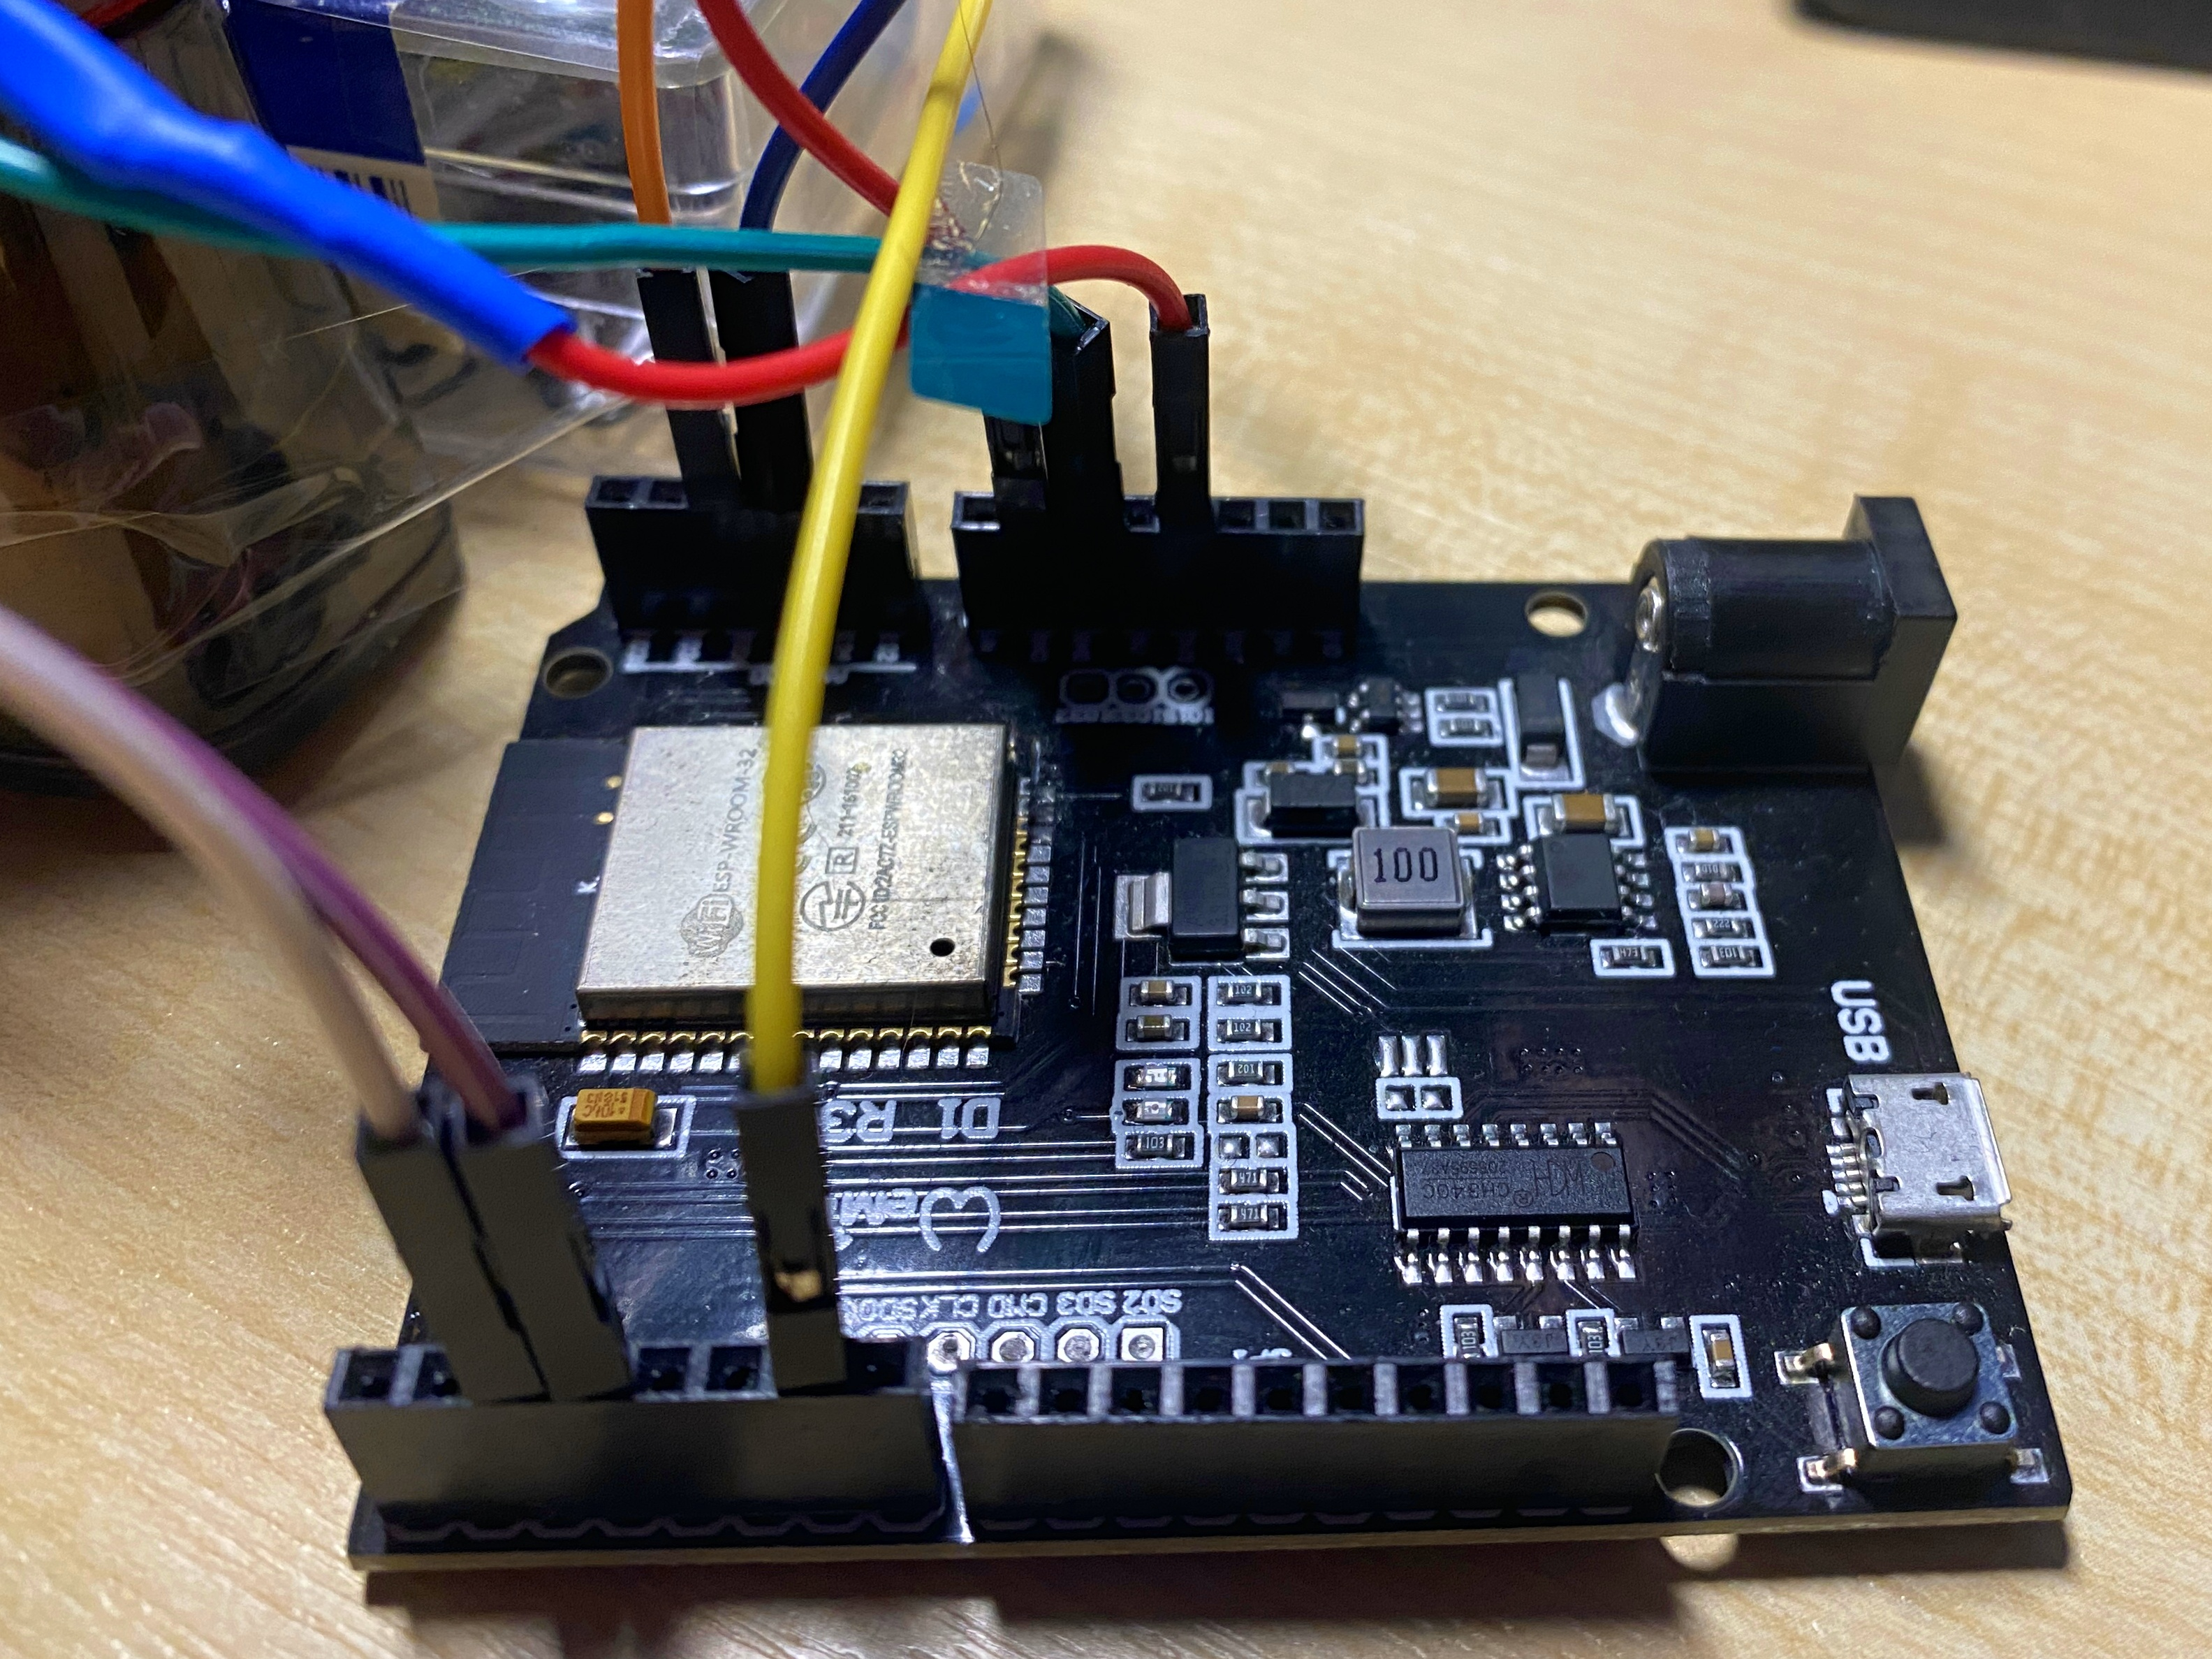
\includegraphics[width=0.9\linewidth]{Obrázky/wiring.JPG}
    \caption{Fotografie zapojení}
    \label{fig:wiring}
\end{figure}

\begin{figure}[H]
    \centering
    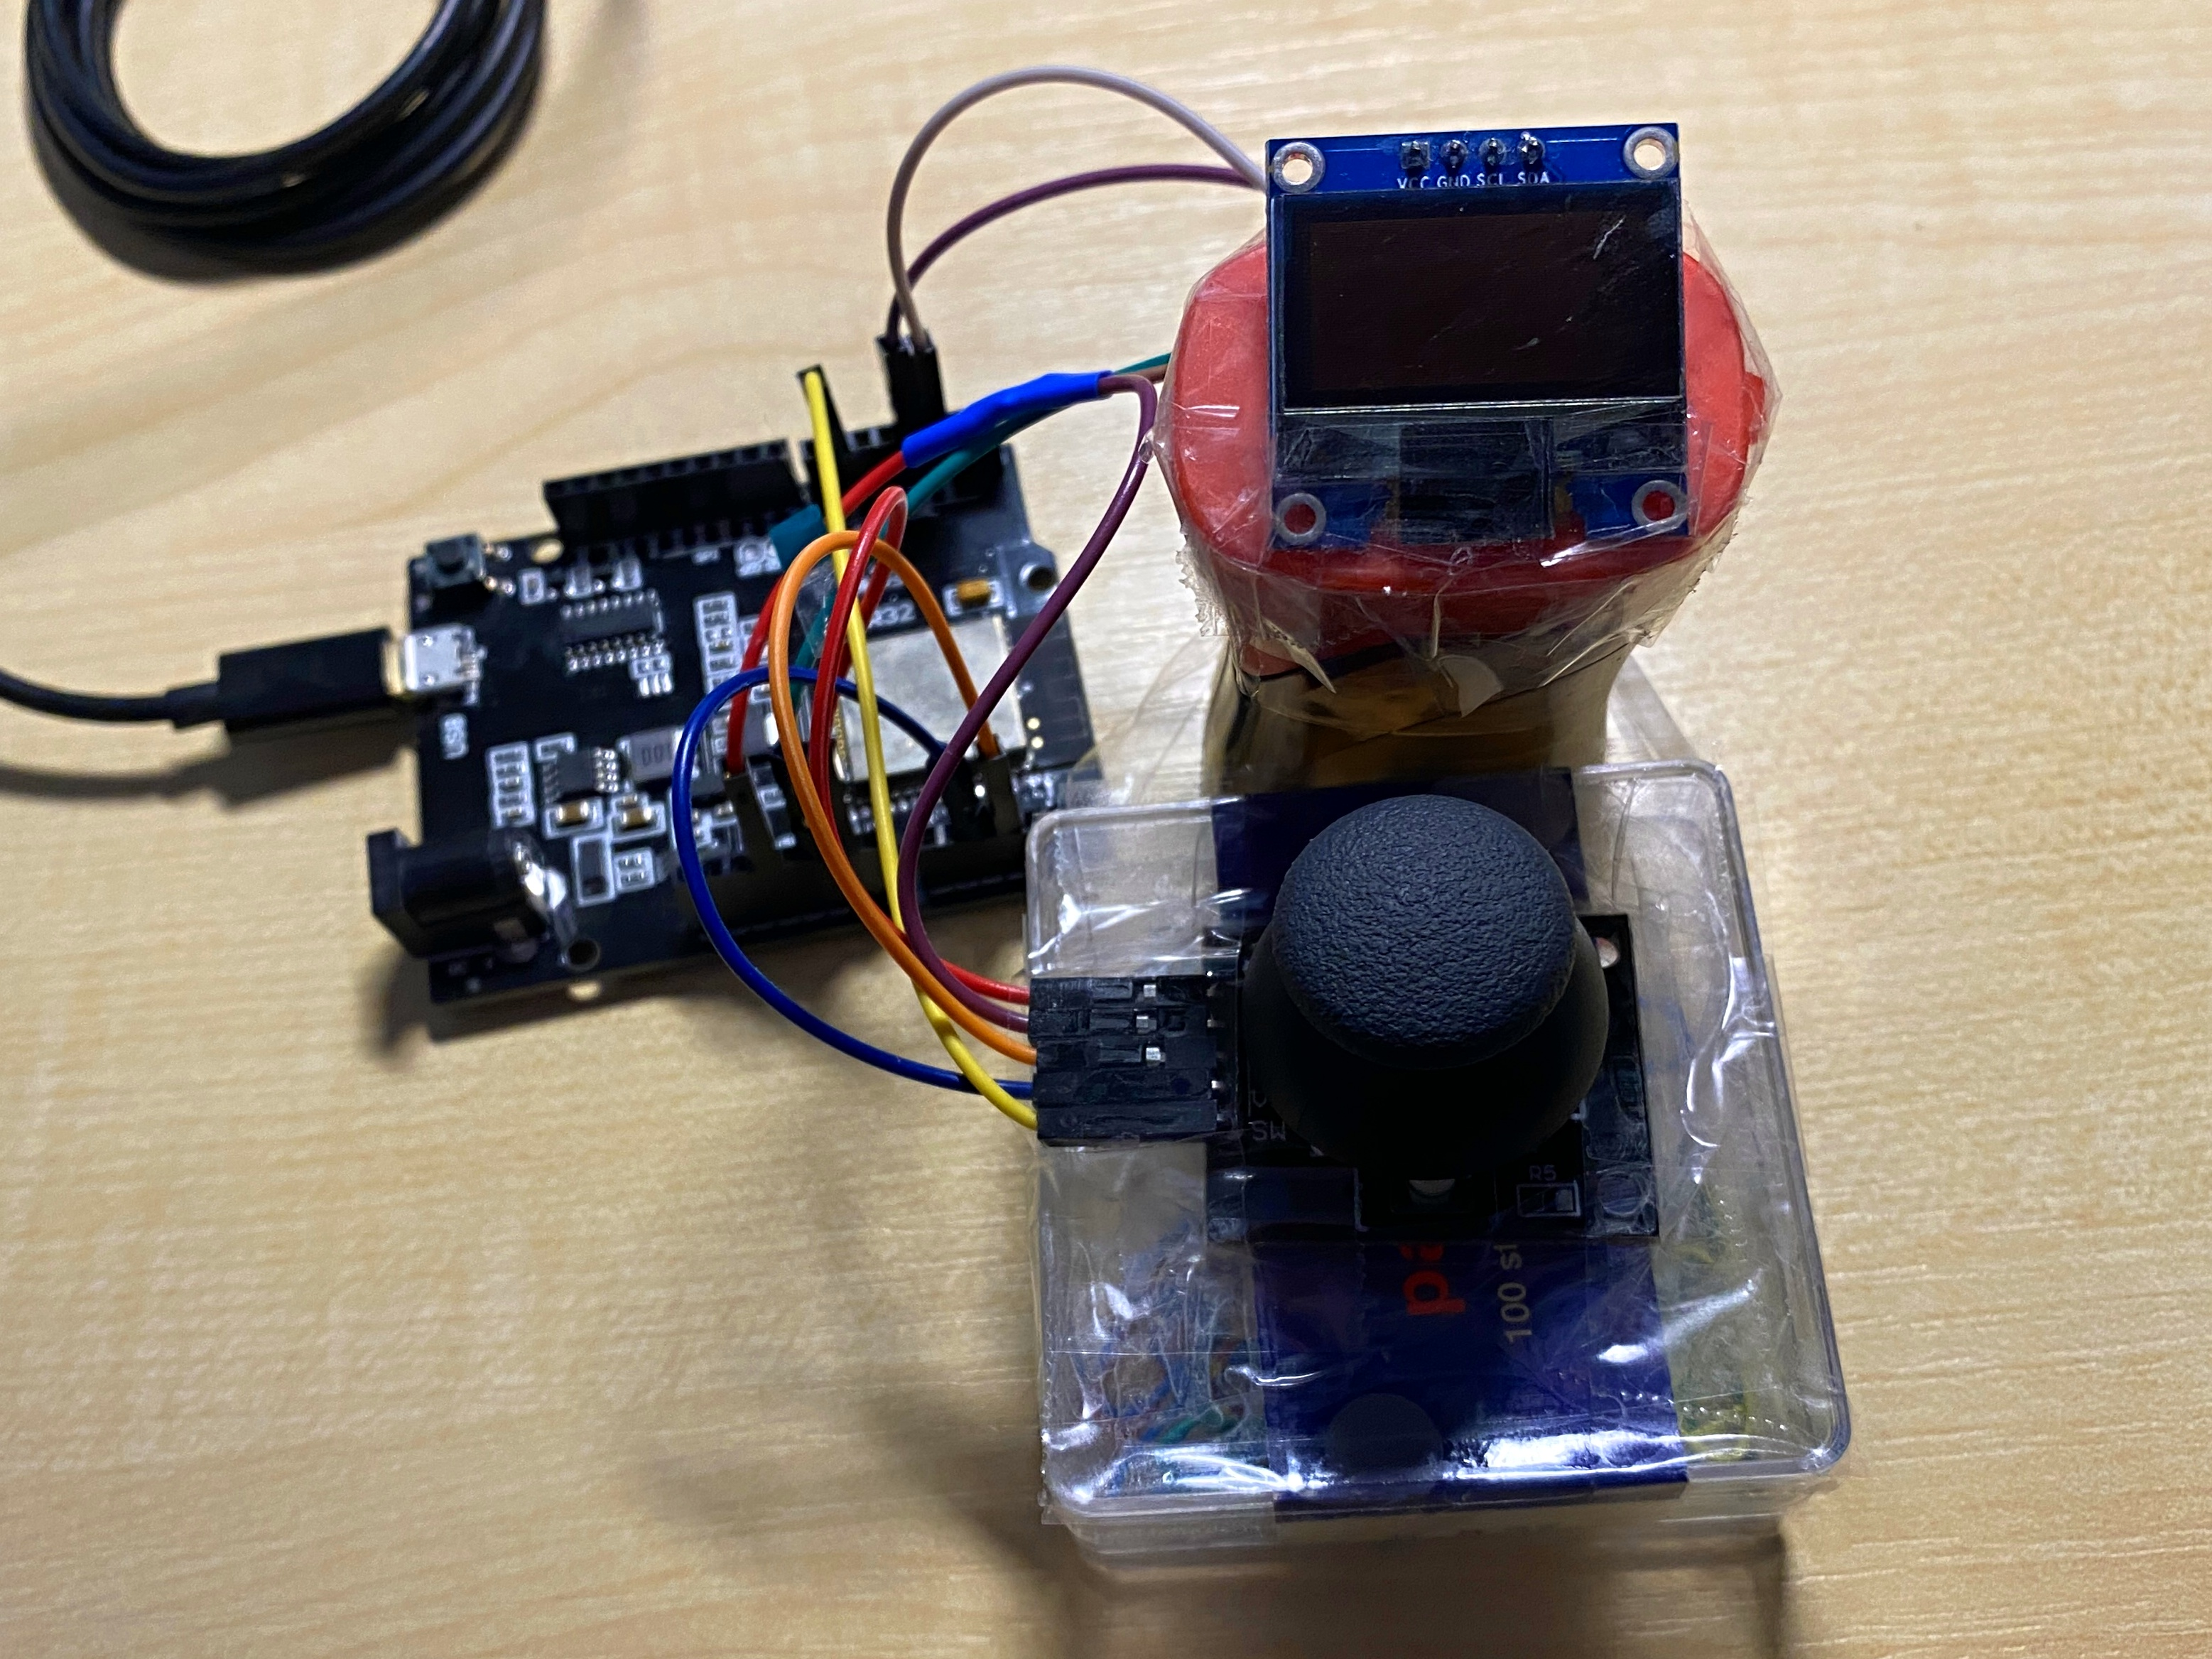
\includegraphics[width=0.9\linewidth]{Obrázky/gameStation.JPEG}
    \caption{Fotografie mé herní stanice}
    \label{fig:gameStation}
\end{figure}

\section{Architektura projektu}

Projekt je v archivu řešen jako jednoduchá, ale čitelně modulární aplikace v ESP-IDF, kde se důsledně odděluje (1) veřejné API jednotlivých modulů (hlavičkové soubory ve složce \texttt{main/public}), (2) implementaci herní logiky a vykreslování (složka \texttt{main/source}), (3) výčtové datové typy (složka \texttt{main/enum}) a (4) struktury reprezentující entity v aplikaci (složka \texttt{main/structure}). Základním vstupním bodem je soubor \texttt{main/main.c}, který obsahuje hlavní smyčku programu realizovanou jako jednoduchý konečný automat v rámci nekonečného cyklu.

Inicializaci $\text{I}^2\text{C}$, OLED displeje, grafického kontextu a vstupních periferií provádím v jim určených zdrojových souborech v rámci dobré praktiky rozdělení na podproblémy.

Nízká vrstva periferií je realizována zdrojovými soubory \texttt{I2C.c} (nastavení master režimu, rychlost a přenosy) a \texttt{SSD1306.c} (inicializační sekvence řadiče, režim zápisu dat a odesílání framebufferu). Na tuto vrstvu navazují moduly \texttt{Graphics} a \texttt{Font5x7}, které poskytují jednotné funkce pro kresbu pixelových entit a textu do framebufferu (tj. kreslí se do RAM a teprve hotový obraz se odešle na displej). Díky tomu je vykreslování deterministické a hra netrpí překreslováním po částech -- v každém snímku se nejdříve složí celá scéna a až poté se přenese na OLED displej.

Herní model je soustředěn ve strukturách ve složce \texttt{main/structure} (např. \texttt{tGame}, \texttt{tBee}, \texttt{tFlower}, \texttt{tSpider}, \texttt{tRaindrop}, \texttt{tPowerUp}) a v enumeracích ve složce \texttt{main/enum} (např. stavový automat hry a typy power-upů). Nad těmito daty pracuje modul \texttt{GameLogic}, který implementuje aktualizační kroky (pohyb, generování objektů, kolize, odpočty efektů, skóre a čas). Samotné zobrazení hry je vyčleněno do modulu \texttt{Renderer}, který z aktuálního stavu \texttt{tGame} sestaví scénu -- vykreslí herní objekty, HUD (skóre/čas) a stavové obrazovky (pauza, game over). Díky takovémuto rozdělení např. změna pravidel hry nevyžaduje zásahy do kreslení a naopak úprava entit či rozložení HUDu nezasahuje do kolizí ani časování, díky tomu jsem hru mohl postupně snadno rozšiřovat.

\section{Zobrazení herního prostředí na OLED displeji}

Veškeré dění hry je vykreslováno na monochromatickém OLED displeji SSD1306 s rozlišením $128\times64$. Herní scéna je složená z jednoduchých pixelových entit a krátkých textových 
informací psané fontem o velikosti $5\times7$. Jednotlivé objekty (včela, květiny, pavouci i power-upy) jsou záměrně kresleny velmi úsporně, aby byly na malém rozlišení dobře čitelné
a hráč na první pohled rozeznal, čemu se vyhýbat a co naopak sbírat.

Hlavní pohyblivou entitou je včela, zobrazovaná jako malý objekt s jednoduchou animací (např. střídání polohy křídel). Květiny jsou vykresleny s odlišnými symboly kvůli rozlišení zdrojové a 
cílové květiny. Pavouci jsou na ploše pouze umístěni a tvoří tak statické překážky, kterým se včela musí vyhnout. Kapky vody padají shora a po zásahu vyvolají dočasné zpomalení včely.
Power-upy (štít a med) jsou zobrazeny vlastní ikonkou a po sebrání se jejich aktivace indikuje symbolem a odpočtem do vypršení efektu. Aktivita štítu je navíc vizualizována kruhem kolem včely a 
zrychlení medem způsobí změnu v animaci křídel.

Kromě herních objektů se na displeji průběžně zobrazuje skóre a zbývající čas a úzký panel, který se plní, když včela sedí na květině, která je zdrojem pylu. Hru je možné také pozastavit. 
Během pauzy se objeví výrazný nápis \uv{PAUSE} a při ukončení hry \uv{GAME OVER} spolu s dosaženým skóre.

Vykreslování je řešeno přes framebuffer. V každém snímku se buffer nejprve vymaže, následně se do něj podle aktuálního stavu hry překreslí všechny entity a výsledná bitmapa se po 
$\text{I}^2\text{C}$ odešle do SSD1306. Přenos kompletního obrazu (1024 B) je dostatečně rychlý na to, aby byl pohyb a animace plynulé a bez viditelného blikání.

Algoritmy pro vykreslování jednotlivých primitiv (bodu, úsečky, kruhu a elipsy) jsou inspirované algoritmy uvedenými na přednáškách předmětu IZG a prakticky implementovaných na cvičeních 
nebo projektu z předmětu IZG. Snažil jsem se také omezit využívání standardních knihovních funkcí jazyka C pro práci s čísly (zejména s plovoucí řádovou čárkou) kvůli lepší optimalizaci -- napsal jsem si vlastní jednoduché matematické funkce, např. na absolutní hodnotu, zaokrouhlování apod. 

\section{Závěr}

Hra na displeji \emph{Bee Pollination} úspěšně demonstruje možnosti mikrokontroléru ESP32 při realizaci interaktivní grafické aplikace. V rámci projektu byla navržena a implementována jednoduchá hra, která však pokrývá široké spektrum úloh: od čtení analogových vstupů a \uv{debouncování} tlačítek, přes řízení grafického OLED displeje po $\text{I}^2\text{C}$ sběrnici, až po zpracování reálného času a kolizní detekce v herní logice. Během vývoje se podařilo vyřešit kalibraci vstupního zařízení (joysticku) a dosáhnout plynulého ovládání, stejně tak jako optimalizovat vykreslování tak, aby i omezené rozlišení 128×64 působilo přehledně a svižně. 


%%%%%%%%%%%%%%%
% Bibliography
%%%%%%%%%%%%%%%

\bibliographystyle{Literatura/czplain}
\renewcommand{\refname}{}
\section{Referenční literatura}
\vspace{-1.1cm}
\bibliography{Literatura/literatura}

\end{document}
